\chapter{Implementacija i korisničko sučelje}
		
		
		\section{Korištene tehnologije i alati}
		
			\textbf{\textit{dio 2. revizije}}
			
			 \textit{Detaljno navesti sve tehnologije i alate koji su primijenjeni pri izradi dokumentacije i aplikacije. Ukratko ih opisati, te navesti njihovo značenje i mjesto primjene. Za svaki navedeni alat i tehnologiju je potrebno \textbf{navesti internet poveznicu} gdje se mogu preuzeti ili više saznati o njima}.
			
			
			\eject 
		
	
		\section{Ispitivanje programskog rješenja}
			
			\textbf{\textit{dio 2. revizije}}\\
			
			 \textit{U ovom poglavlju je potrebno opisati provedbu ispitivanja implementiranih funkcionalnosti na razini komponenti i na razini cijelog sustava s prikazom odabranih ispitnih slučajeva. Studenti trebaju ispitati temeljnu funkcionalnost i rubne uvjete.}
	
			
			\subsection{Ispitivanje komponenti}
			\textit{Potrebno je provesti ispitivanje jedinica (engl. unit testing) nad razredima koji implementiraju temeljne funkcionalnosti. Razraditi \textbf{minimalno 6 ispitnih slučajeva} u kojima će se ispitati redovni slučajevi, rubni uvjeti te izazivanje pogreške (engl. exception throwing). Poželjno je stvoriti i ispitni slučaj koji koristi funkcionalnosti koje nisu implementirane. Potrebno je priložiti izvorni kôd svih ispitnih slučajeva te prikaz rezultata izvođenja ispita u razvojnom okruženju (prolaz/pad ispita). }
			
			
			
			\subsection{Ispitivanje sustava}
			
			 \textit{Potrebno je provesti i opisati ispitivanje sustava koristeći radni okvir Selenium\footnote{\url{https://www.seleniumhq.org/}}. Razraditi \textbf{minimalno 4 ispitna slučaja} u kojima će se ispitati redovni slučajevi, rubni uvjeti te poziv funkcionalnosti koja nije implementirana/izaziva pogrešku kako bi se vidjelo na koji način sustav reagira kada nešto nije u potpunosti ostvareno. Ispitni slučaj se treba sastojati od ulaza (npr. korisničko ime i lozinka), očekivanog izlaza ili rezultata, koraka ispitivanja i dobivenog izlaza ili rezultata.\\ }
			 
			 \textit{Izradu ispitnih slučajeva pomoću radnog okvira Selenium moguće je provesti pomoću jednog od sljedeća dva alata:}
			 \begin{itemize}
			 	\item \textit{dodatak za preglednik \textbf{Selenium IDE} - snimanje korisnikovih akcija radi automatskog ponavljanja ispita	}
			 	\item \textit{\textbf{Selenium WebDriver} - podrška za pisanje ispita u jezicima Java, C\#, PHP koristeći posebno programsko sučelje.}
			 \end{itemize}
		 	\textit{Detalji o korištenju alata Selenium bit će prikazani na posebnom predavanju tijekom semestra.}
			
			\eject 
		
		
		\section{Dijagram razmještaja}
			
			Dijagram rasporeda ilustrira kako su fizički i softverski resursi distribuirani unutar operativnog okvira sustava. Na serveru se smještaju dva ključna servisa: servis za web i servis za upravljanje bazom podataka. Kroz web preglednike, korisnici stječu pristup funkcionalnostima web aplikacije. Ovaj sustav funkcioniše po modelu klijent-server arhitekture gdje je komunikacijski protokol između korisničkih uređaja i servera omogućen putem HTTP veze.

		\begin{figure} [H]
			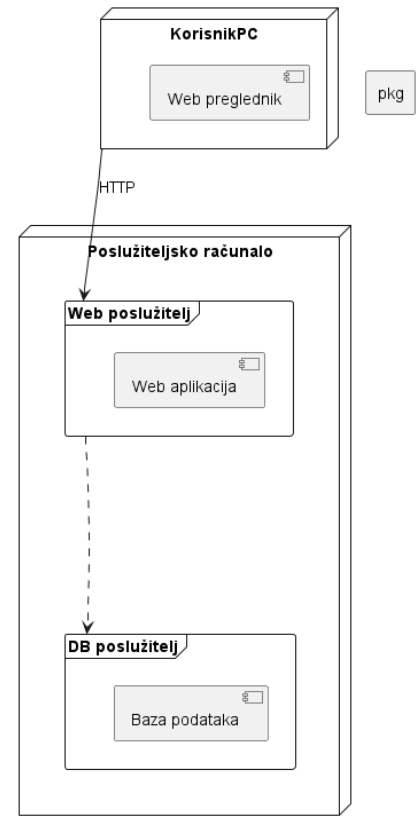
\includegraphics[width=1\linewidth]{slike/dijagramRazmjestanja.png}
	        \centering
	        \caption{Prikaz dijagrama razmještanja}
	        \label{fig:Prikaz dijagrama razmještanja}
        \end{figure}

			\eject 
		
		\section{Upute za puštanje u pogon}

		Za postavljanje aplikacije u produkcijsko okruženje, ključno je implementirati sve komponente na GitHub platformi. Ovaj korak je presudan jer omogućava kreiranje Docker kontejnera, koji su esencijalni za funkcionalnost aplikacije u radnom okruženju. Izvorni kod naše aplikacije dostupan je na https://github.com/KvesaFer/Codeblaze.

		Implementaciju aplikacije izvodimo kroz Render, cloud-based platformu-as-a-service (PaaS). Render nudi potrebnu infrastrukturu za pokretanje aplikacije. Prije početka rada na Render platformi, neophodno je u korijenskom direktoriju izvornog koda kreirati 'render.yaml' datoteku. Ova datoteka služi kao 'Blueprint spec', konfiguracijski set za implementaciju i aktivaciju aplikacije na Render platformi.

		U 'render.yaml' datoteci definiramo tri ključna servisa naše aplikacije: 'server', 'client', i 'db'. Svaki servis, osim PostgreSQL baze, treba sadržavati atribute 'type', 'name', i 'env'. Za PostgreSQL bazu, potrebno je navesti samo 'name', a detalji implementacije su već dostupni kroz predefiniranu uslugu na Render platformi.

		Dodatno, definiramo svojstva za preostale servise - frontend i backend. Atribut 'env' određuje okruženje izvođenja i postavljen je na 'Docker', što omogućava izgradnju aplikacije kroz Docker kontejnere. Svaki definirani servis predstavlja zasebnu 'Docker image' datoteku, koja uključuje kod, alate, biblioteke i ostale postavke potrebne za izgradnju kontejnera.

		Za svaki servis, 'repo' svojstvo postavljamo na putanju GitHub repozitorija s izvornim kodom aplikacije. Također, definiramo 'branch' svojstvo na 'main' granu i 'rootDir' za određivanje korijenskog direktorija repozitorija. 'BuildFilter' svojstvo omogućava definiranje putanje do datoteka čije promjene na 'main' grani iniciraju redeployment servisa.

		Za postavljanje varijabli okruženja, koristimo mogućnost definiranja zavisnosti varijabli jednog servisa o svojstvima već postojećih Render servisa. Varijable okruženja za 'backend' servis povezan s bazom podataka dohvaćamo preko definiranih svojstava Render servisa za PostgreSQL bazu. Ostale varijable, koje su privatne, postavljamo direktno na Render platformu.

		Kreiranje korisničkog računa i prijava na https://dashboard.render.com/ su prvi koraci za korištenje platforme. Nakon toga, odabiremo 'Blueprints' i 'New Blueprint Instance', birajući repozitorij i granu s našim 'render.yaml' datotekom. Render omogućava povezivanje s GitHub računom i odabir repozitorija.

		Nakon spremanja promjena, Render web aplikacija postaje povezana s repozitorijem koji sadrži izvorni kod i 'render.yaml' datoteku. Na osnovu definirane konfiguracije, Render potom pokreće aplikaciju u radno okruženje.

		Konačna verzija aplikacije dostupna je na URL-u koji se generira nakon uspješnog deploya na Render platformi. Važno je napomenuti da, u skladu s uputama za deploy, potrebno je uključiti specifične konfiguracijske korake. To uključuje dodavanje Dockerfile-a, koji se nalazi u 'docker' direktoriju, sa specifičnim verzijama za Maven i Gradle. Također, preporučuje se postavljanje 'server.servlet.context-path' na '/api' u 'application.properties' za backend zahtjeve.

		Za lokalni razvoj, koristeći Liquibase i H2 bazu, preporuča se dodavanje odgovarajućih dependency-a u 'pom.xml' i kreiranje 'application-dev.properties' za lokalni dev profil. Ovo olakšava razvoj i testiranje aplikacije. Važno je paziti na promjene nad bazom, gdje se promjene nad changelogovima ne smiju mijenjati jednom kada su deployani.

		Kreiranje baze podataka na Renderu uključuje postavljanje imena baze te postavljanje opcionalnog korisničkog imena, dok je lozinka automatski generirana. Također, konfiguracija backenda i frontenda na Renderu zahtijeva povezivanje GitHub računa, odabir projekta, postavljanje environment varijabli, i konfiguraciju Dockerfile-a.

		Za deploy frontenda, koraci uključuju dodavanje potrebnih dependency-a u 'package.json', konfiguraciju proxy servera, i postavljanje build i start skripti. Konačno, aplikacija će biti dostupna na URL-u koji se generira nakon deploya na Render platformi.

		Konačna aplikacija dostupna je na poveznici:

		\eject